% !TEX root = ../IntroImaging.tex


\chapter{Sparsity, Inverse Problems and Compressed Sensing}
\label{chap-sparsity}

Current standards for compressing music, image or video (MP3, JPG, or MPEG) all use methods derived from non-linear approximation. These methods compute an approximation of the initial data using a linear combination of a small number of elementary functions (such as sinusoids or wavelets).
%
These methods, initially used for approximation, denoising or compression, have been applied more recently to more difficult problems, such as increasing the resolution or inversion of operators in medical imaging. These extensions require the resolution of large-scale optimization problems, and are the subject of intense research activity.
%
One of the most recent advances in this field, compressed sampling, uses the theory of random matrices in order to obtain theoretical guarantees for the performance of these techniques. Compressed sampling allows Claude Shannon's theory of sampling and compression to be considered from a new angle. The compressibility of the data allows for simultaneous sampling and compression.

This chapter presents the key mathematical concepts that have allowed evolution from classical Shannon sampling to compressed sampling. The notion of sparse decomposition, which makes it possible to formalize the idea of compressibility of information, is the main thread.


%%%%%%%%%%%%%%%%%%%%%%%%%%%%%%%%%%%%
\section{Traditional Sampling}
\label{sec-sampling}

In the digital world, most data (sound, image, video, etc.) are discretized in order to store, transmit and modify them.
%
From an analog signal, which is represented by a continuous function $s \mapsto \tilde f(s)$, the measurement device calculates a set of discretized values $f = (f_q)_{q=1}^Q \in \RR^Q$.
%
Thus, $Q$ is the number of time samples for an audio piece or the number of pixels for an image.
%
Figure~\ref{fig-samples} shows examples of discretized data.
%
In the case of an image, $\tilde f(s)$ represents the amount of light arriving at a point $s \in \RR^2$ of the camera's focal plane, and $f_q = \int_{c_q} \tilde f(s) \text{d} s$ is the total amount of light illuminating the $c_q$ surface of a CCD sensor indexed by $q$.
%
For simplicity, here we assume scalar data (eg mono sound, grayscale image, or video), but the techniques described here may extend to vector data (stereo sound, color image ).


\begin{figure} \centering
\begin{tabular}{@{}c@{\hspace{5mm}}c@{}}
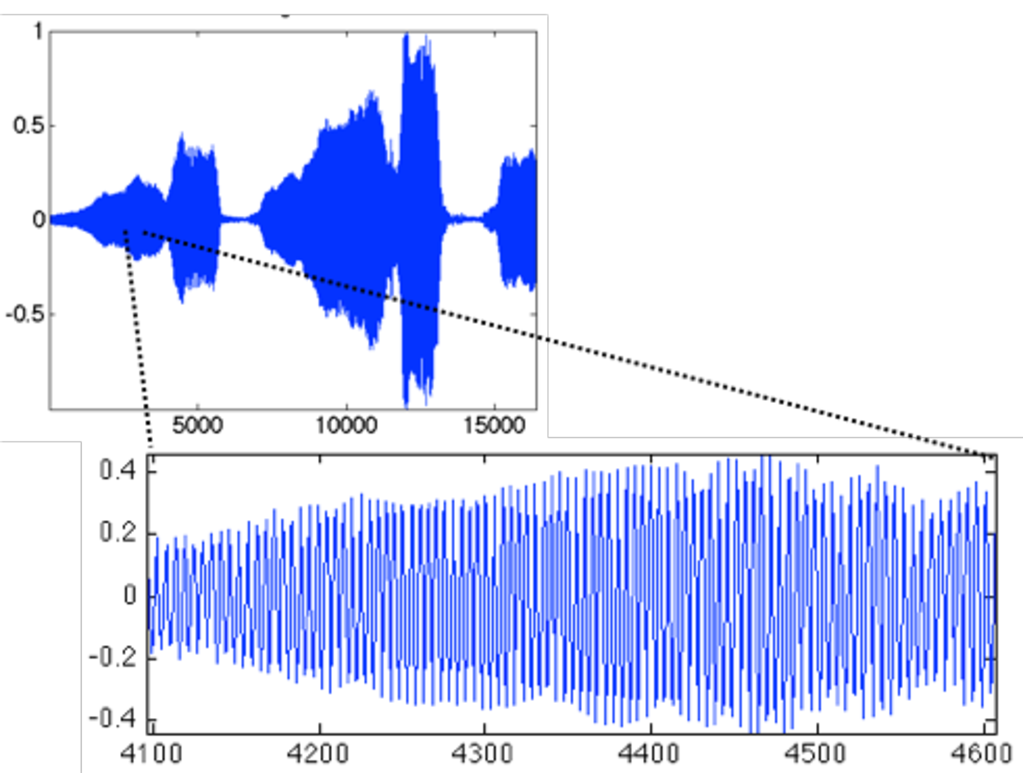
\includegraphics[width=.45\linewidth]{discrete/signal} &
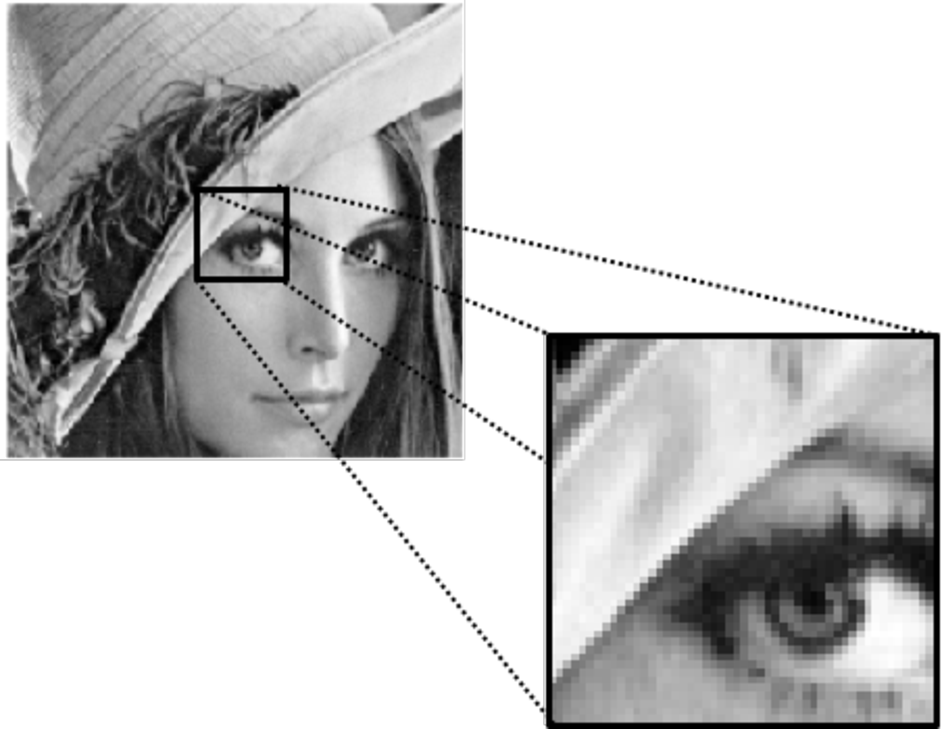
\includegraphics[width=.45\linewidth]{discrete/image}
\end{tabular}
\caption{\label{fig-samples} Examples of a sound signal (1D data) and an image (2D data) discretized.}
\end{figure}

It is the theory developed by Claude Shannon~\cite{Shannon1948} that laid the foundation for sampling (the use of a discrete vector $f$ to faithfully represent a continuous function $\tilde f$) but also those of lossless compression.
%
We will see how current research has made it possible to build on these foundations lossy compression methods (i.e with a slight degradation of the quality), as well as to revisit the conventional sampling to give rise to the idea of compressed sampling.


%%%%%%%%%%%%%%%%%%%%%%%%%%%%%%%%%%%%
\section{Nonlinear Approximation and Compression}


%%%%%
\subsection{Nonlinear Approximation}

The size $Q$ of these data is generally very large (of the order of million for an image, of the billion for a video) and it is necessary to calculate a more economical representation in order to be able to store $f$ or to transmit it on a network.
%
All modern lossy compression methods (MP3, JPEG, MPEG, etc.) use sparse decompositions (that is composed of few non-zero coefficients) in a dictionary $\Psi = (\psi_n)_{n=1}^N$ composed of elemental atoms $\psi_n \in \RR^Q$.
%
It is thus sought to approach $f$ with the aid of a linear combination
\eq{
	f \approx  \Psi x \eqdef \sum_{n=1}^N x_n \psi_n \in \RR^Q
}
where the $x = (x_n)_{n=1}^N \in \RR^N$ are the coefficients that will be stored or transmitted. In order for this representation to be economical, and for storage to take up little space, it is necessary that a maximum of coefficients $x_n$ be zero, so that only the non-zero coefficients have to be stored. Given a budget $M>0$ of non-zero coefficients, the best possible combination is sought in order to approximate $\ell^2$ the initial data. The aim is to solve the optimization problem
\eql{\label{eq-pbm-approx}
	x^\star \in \uargmin{x \in \RR^N} \enscond{  \norm{f - \Psi x}_2  }{ \norm{x}_0 \leq M }
	\qwhereq
	\norm{f}_2^2 \eqdef \sum_{q=1}^Q |f_q|^2.
}
Here we have noted $\norm{x}_0 \eqdef \sharp\enscond{n}{x_n \neq 0}$ the number of non-zero coefficients of $x$, which is a counting measure often referred to by language abuse as the \guill{pseudo-norm} $\ell^0$ (which is not a standard!). This abuse of language will be explained in section~\ref{sec-pb-inv}, see in particular figure~\ref{fig-boules}.

The problem~\eqref{eq-pbm-approx} is in general impossible to solve: it is a combinatorial problem, which, without further hypothesis on $\Psi$, requires the exploration of all combinations of $M$ coefficients non-zero. It has been proved that this problem is indeed NP-difficult~\cite{Natarajan95}.


%%%%%
\subsection{Approximation in an orthonormal basis}

There is however a simple case, which is very useful for compression: this is the case where $\Psi$ is an orthonormal basis of $\RR^Q$, ie $Q = N$ and
\eq{
	\dotp{\psi_n}{\psi_{n'}} = \choice{
		1 \qsiq n = n', \\
		0 \quad\text{sinon.}
	}
	\qwhereq
	\dotp{f}{g} \eqdef \sum_{q=1}^Q f_q g_q.
}
This case is the one most often encountered for data compression, using for example discrete Fourier orthogonal bases, local cosines (used for MP3, JPG and MPG) and wavelets (used for JPEG2000), see the book~\cite{mallat2009a-wav}.
%
In this case, we have the identity of Parseval which corresponds to the decomposition of $f$ in an orthonormal basis
\eql{\label{eq-expansion-bon}
	f = \sum_{n=1}^N \dotp{f}{\psi_n} \psi_n 
	\qetq
	\norm{f - \Psi x}_2^2 = \sum_{n=1}^N | \dotp{f}{\psi_n} - x_n |^2.
}
These formulas show that the solution of~\eqref{eq-pbm-approx} is very simple to calculate.
%
Indeed, to minimize $\norm{f - \Psi x}_2$, for each non-zero $x_n$, one should choose $x_n = \dotp{f}{\psi_n}$.
%
And since we set a maximum budget of $M$ non-zero coefficients, we must choose the $M$ largest coefficients $|\dotp{f}{\psi_n}|$ in the formula~\eqref{eq-expansion-bon}. Mathematically, if we note $|\dotp{f}{\psi_{n_1}}| \geq |\dotp{f}{\psi_{n_2}}| \geq \ldots$ a sorting of the coefficients in descending order, then a $x^\star$ solution of~\eqref{eq-pbm-approx} is given by
\eql{\label{eq-formule-thresh}
x^\star_n = \choice{
\dotp{f}{\psi_{n}} \qsiq \in \{n_1,\ldots, n_M\}, \\
0 \quad\text{otherwise}
}
}

\newcommand{\myPic}[1]{\includegraphics[trim=50 50 30 30,clip,width=.24\linewidth]{approx/#1}}
\begin{figure}\centering
\begin{tabular}{@{}c@{\hspace{1mm}}c@{\hspace{1mm}}c@{\hspace{1mm}}c@{}}
\myPic{cameraman} &
\myPic{cameraman-4} &
\myPic{cameraman-8} &
\myPic{cameraman-16} \\
$f$ & 
$\Psi x^\star, M=N/4$ & 
$\Psi x^\star, M=N/8$ &  
$\Psi x^\star, M=N/16$ 
\end{tabular}
\caption{\label{fig-approx} Approximate Examples $f \approx \Psi x^\star$ with $M = \norm{x^\star}_0$ which varies, for a $f \in \RR^N$ image of $N = 256^2$ pixels.}
\end{figure}


The figure~\ref{fig-approx} shows approximations $f \approx \Psi x^\star$, with a variable number $M = \norm{x^\star}_0$  of coefficients.
%
These approximations are performed using an orthogonal base of wavelets $\Psi$, called the Daubechies 4 base, which are similar to the functions used in the JPEG2000 image compression standard, and are popular because there is a fast algorithm for calculate the scalar products $( \dotp{f}{\psi_{n}} )_n$ with a computation time proportional to $Q$ (see the book~\cite[Chapter 7]{mallat2009a-wav} for a complete description of the theory of wavelets).
%
It can be seen that the quality of the reconstructed image $\Psi x^\star$ degrades when $M$ decreases, but one can still considerably reduce the amount of information to be stored (the $M/Q$ compression ratio is small), while maintaining an acceptable visual quality.
%
This fundamental observation corresponds to the fact (observed in practice) that natural images are very well approximated by a \guill{sparse} linear combination of the form $\Psi x^\star$ with $\norm{x^\star}_0 \leq M$.
%
It is important to note that, although the calculation of $\Psi x^\star$ from $x^\star$ is a linear formula, the calculation of $x^\star$ from $f$ is \textit{non-linear}, as can be seen in the formula~\eqref{eq-formule-thresh}. The transition from $f$ to its approximation $\Psi x^\star$ is called a non-linear approximation.
%
The theoretical justification of this observation is the object of the study of nonlinear approximation theory, which seeks to prove that $\norm{f-\Psi x^\star}$ decreases rapidly when $M$ increases under certain assumptions of regularity over $f$, for instance assuming that the image is piecewise smooth, see~\cite[Chap. 9]{mallat2009a-wav}.

In order to obtain an complete compression algorithm, it is then necessary to use a technique making it possible to convert the $M$ coefficients $(x_{n_1}, \dots, x_{n_2})$ into binary writing and also to store the non-zero indices $(n_1,\ldots, n_M)$. This is done simply using techniques derived from information theory, in particular entropy coding methods, see~\cite[Chap. 10]{mallat2009a-wav}.

%%%%%%%%%%%%%%%%%%%%%%%%%%%%%%%%%%%%%%%%%%%%%
\section{Inverse Problems and Sparsity}
\label{sec-pb-inv}

%%%%%
\subsection{Inverse Problems}

Before $f$ data can be stored, it is most of the time necessary to carry out a preliminary restoration step, which consists in improving the quality of the data from observations of low quality, that is to say --9 of low resolution, possibly blurred , entangled with errors and noisy. In order to take into account the whole chain of data formation, we model mathematically the acquisition process in the form
\eql{\label{eq-fwd-model}
	y = \Phi f + w \in \RR^P
}
where $y \in \RR^P$ are the $P$ observations measured by the device, $w \in \RR^P$ is a measurement noise (unknown), $f \in \RR^Q$ is the image (unknown) that one wishes to recover, and $\Phi : \RR^Q \rightarrow \RR^P$ is an operator modeling the acquisition apparatus, and which is assumed to be ``linear". This means that $\Phi$ may be considered as a (gigantic) matrix $\Phi \in \RR^ (P \times Q) $. It is important to note that most of the time this matrix $\Phi$ is never explicitly stored, it is manipulated implicitly by means of fast operations (convolution, masking, etc.).


\begin{figure} \centering
\begin{tabular}{@{}c@{\hspace{4mm}}c@{\hspace{4mm}}c@{}}
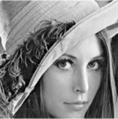
\includegraphics[width=.25\linewidth]{operators/lena-original} &
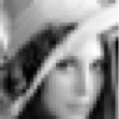
\includegraphics[width=.25\linewidth]{operators/lena-blurring} &
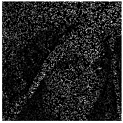
\includegraphics[width=.25\linewidth]{operators/lena-inpainting} \\
Image originale $f$ & $\Phi f$ (flou) & $\Phi f$ (masquage)  
\end{tabular}
\caption{Observation (noiseless, $w=0$) $y=\Phi f$ in the case of a convolution ($\Phi f = \phi \star f$ is a convolution against a low pass filter $\phi$) and missing data  ($\Phi=\diag(\mu_q)_{q=1}^Q$ is a masking operator).  \label{fig-exemple-ip} }
\end{figure}


This model, which may seem rather restrictive (in particular the hypothesis of linearity) makes it possible to model a surprising quantity of situations that one meets in practice. For example,
\begin{itemize}
	\item Denoising: $\Phi = \Id_{\RR^Q} $, $P = Q$ and one is in the (simplest) situation in which one only seeks to remove the noise $w$ ;
	 \item Deconvolution: (see Figure~\eqref{fig-exemple-ip}, center) $\Phi f = \phi \star f$ is a convolution by a filter $\phi$ modeling for example the blur of a camera (either a blur of shake or a blur due to development) ;
	\item Missing data: (see Figure~\eqref{fig-exemple-ip}, right)  $\Phi=\diag(\mu_q)_{q=1}^Q$  is a diagonal masking operator, such as $\mu_q = 1$ if the data indexed by $q$ (for example, one pixel) is observed, and $\mu_q = 0$ if the data is missing;
	 \item tomographic imagery: $\Phi$ is a more complex linear operator, calculating integrals along straight lines (the Radon transform), see \cite[Sect. 2.4]{mallat2009a-wav}.
\end{itemize}
There are many other examples (in medical imaging, seismic, astrophysics, etc.), and in each case, calculating a good approximation of $f$ from $y$ is very difficult. Indeed, with the exception of denoising (ie $\Phi = \Id_{\RR^Q} $), the formula $\Phi^{-1} y = f + \Phi^{-1} w$ can not be used either because $\Phi$ is not invertible (for example for missing data), or because $\Phi$ has very small eigenvalues (for deconvolution or tomography), so that $\Phi^{-1} w$ is going to be very large, and thus $\Phi^{-1} y$ is a very bad approximation of $f$.


%%%%%
\subsection{Sparse Regularization}

To remedy this problem, we need to replace $\Phi^{-1}$ with an approximate \guill{inverse} which takes into account additional assumptions about the $f$ signal we are looking for. Recent methods, which give the best results on complex data, use an approximate inverse which is nonlinear. This may seem contradictory because $\Phi$ is linear, but the use of nonlinear methods is crucial to take advantage of realistic assumptions about complex data such as images.
%
Based on the approximation and compression techniques discussed in the previous section, current methods seek to exploit the fact that one can approach $f$ with a sparse approximation $\Psi x$ with $\norm{x}_0 \leq M$. Given a parameter $M> 0$, we will look to approximate $f$ by $f^\star = \Psi x^\star$ where $x^\star$ is a solution of
\eql{\label{eq-pbm-l0}
	x^\star \in \uargmin{x \in \RR^N} \enscond{\norm{y - \Phi \Psi x}_2}{\norm{x}_0 \leq M}
}
We see that~\eqref{eq-pbm-l0} is quasi-identical to~\eqref{eq-pbm-approx}, except that $f \in \RR^Q$ (unknown) has been replaced by $y\in \RR^P$, and that matrix $\Psi \in \RR^{Q \times N}$ by matrix product $\Phi \Psi \in \RR^{P \times N} $. In the particular case of denoising, $\Phi = \Id_{\RR^Q} $, the problems~\eqref{eq-expansion-bon} and~\eqref{eq-pbm-l0} are equivalent and have the same solution, so that the nonlinear approximation solves the denoising problem .

In the case of any operator $\Phi$, the problem~\eqref{eq-pbm-l0} is however an optimization problem extremely difficult to solve. Indeed, even if $\Psi$ is an orthonormal basis, in general (except in the case of denoising $\Phi = \Id_{\RR^Q}$), the matrix $\Phi \Psi$ is not orthogonal, so that the formula~\eqref{eq-formule-thresh} is not applicable, and~\eqref{eq-pbm-l0} is a NP-difficult combinatorial search problem.


%%%%%
\subsection{$\ell^1$ Regularization}

The approximation of the solutions of the problem~\eqref{eq-pbm-l0} using efficient methods is one of the most active subjects of research in data processing (and more generally in applied mathematics, imagery, statistics and machine learning). There are many methods, including greedy algorithms (see, for example,~\cite{MallatMP}) and convex relaxation methods. We will focus on this second class of methods.
%
One way (heuristic) to introduce these techniques is to replace $\norm{\cdot}_0$ in the~\eqref{eq-pbm-l0} problem with the function $\norm{\cdot}_\al^\al$, which is set to $\al>0$ by
\eq{
	\norm{x}_{\al}^\al \eqdef \sum_{n=1}^N |x_n|^\al.
}
Figure \ref{fig-boules} shows in the (unrealistic but convenient to draw) case of $N = 2$ coefficients, the balls of the $B_\al \eqdef \enscond{x}{\norm{x}_\al \leq 1}$ units associated with these functional $\norm{\cdot}_\al$. It can thus be seen that $B_\al$ \guill{tend} to the \guill{unit ball} associated with the counting measure $\norm{\cdot}_0$ as $\al$ tends to $0$,
\eq{
	B_\al \overset{\al \rightarrow 0}{\longrightarrow} B_0 \eqdef \enscond{ x \in [-1,1]^N }{ \norm{x}_0 \leq 1 },
}
the convergence of these sets (which is well visualized in the figure) being in the sense for example of the Hausdorff distance.
%
The limiting ball $B_0$ is composed of extremely sparse vectors, since they are composed of a single non-zero component.

\begin{figure} \centering
\begin{tabular}{@{}c@{\hspace{1mm}}c@{\hspace{1mm}}c@{\hspace{1mm}}c@{\hspace{1mm}}c@{}}
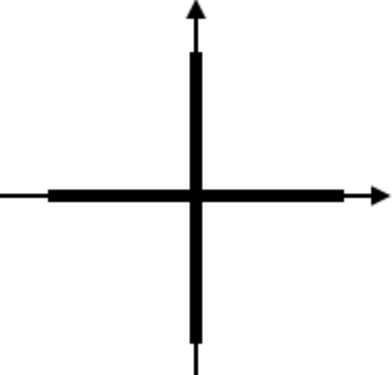
\includegraphics[width=.19\linewidth]{balls/l0} &
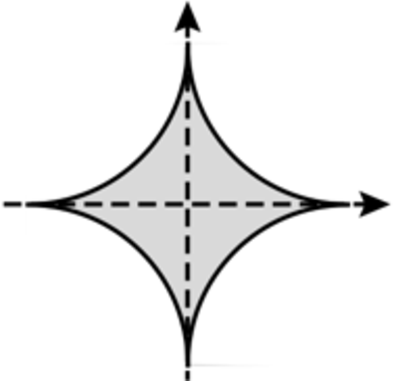
\includegraphics[width=.19\linewidth]{balls/l12} &
\includegraphics[width=.19\linewidth]{balls/l1} &
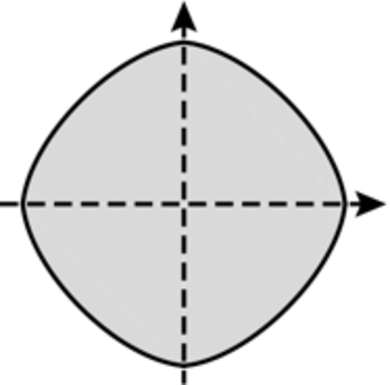
\includegraphics[width=.19\linewidth]{balls/l32} &
\includegraphics[width=.19\linewidth]{balls/l2} \\
$\al=0$ & $\al=1/2$ & $\al=1$ & $\al=3/2$ & $\al=2$
\end{tabular}
\caption{\label{fig-boules} Balls $B_\al$ for different values of $\al$.}
\end{figure}


One then has to take into account two conflicting points to choose a value of $\al$:
\begin{itemize}
	\item In order to have a functional enforcing the sparsity of vectors, we want to use a value of $\al$ as low as possible to replace $\norm{\cdot}_0$ by $\norm{\cdot}_\al$.
	\item In order to calculate the solution of~\eqref{eq-pbm-l0} with $\norm{\cdot}_\al$ instead of $\norm{\cdot}_0$, it is important that the $\norm{\cdot}_\al$ be \textit{convex}. The convexity is indeed essential in order to obtain a problem that is not NP-difficile and to be able to benefit from fast calculation algorithms. These algorithms find an exact solution $x^\star$ in polynomial time or quickly converge to this solution.
\end{itemize}
The convexity constraint of $\norm{\cdot}_\al$ requires that the set $B_\al$ be convex, which equivalently means that $\norm{\cdot}_\al$ must be a \textit{norm}. This imposes that $\al \geq 1$. Taking these two constraints into account leads naturally to the choice  $\al = 1$, so that we consider the convex optimization problem (that is, seeks to minimize a convex function on a convex set)
\eql{\label{eq-pbm-l1}
	x^\star \in \uargmin{x \in \RR^N} \enscond{  \norm{y - \Phi \Psi x}_2  }{ \norm{x}_1 = \sum_{n=1}^N |x_n| \leq \tau }, 
}
so that the retrieved image is defined as $f^\star = \Psi x^\star$.
%
It may be noted that a parameter $\tau>0$ was used here, which plays a role similar to parameter $M$ which appears in~\eqref{eq-pbm-l0}.
%
The question of choosing this parameter $\tau$ is crucial. If the noise $w$ is small, then we want that $\Phi f^\star = \Phi\Psi x^\star$ be close to $y$, and so we will choose $\tau$ big. On the contrary, if the noise $w$ is important, in order to obtain a greater denoising effect, the value of $\tau$ is reduced. The choice of a $\tau$ \guill{optimal} is a difficult search problem, and there is no universal response, the existing strategies strongly depend on the $\Phi$ operator as well as the atoms family~$\Psi$ .

The problem~\eqref{eq-pbm-l1} was initially proposed by engineers in the fields of seismic imaging (see for example~\cite{santosa1986linear}), and it was introduced jointly in signal processing under the name \guill{basis pursuit}~\cite{chen1999atomi} and in statistics under the name \guill{Lasso}~\cite{tibshirani1996regre}.


\begin{figure} \centering
\begin{tabular}{@{}c@{\hspace{4mm}}c@{\hspace{4mm}}c@{}}
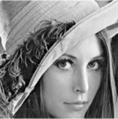
\includegraphics[width=.25\linewidth]{operators/lena-original} &
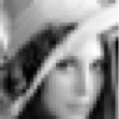
\includegraphics[width=.25\linewidth]{operators/lena-blurring} &
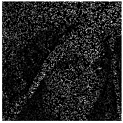
\includegraphics[width=.25\linewidth]{operators/lena-inpainting} \\
$f$ Original & Observations $y$ & Reconstruction $f^\star$
\end{tabular}
\caption{Examples of reconstruction with missing data, $\Phi = \diag(\mu_q)_{q = 1}^Q$ with $\mu_q \in \{0,1\}$ and a number of observed data $\sharp\enscond{q}{\mu_q = 1}=10\%$. \label{fig-inpainting}}
\end{figure}

The problem~\eqref{eq-pbm-l1}, although convex, remains a difficult problem to solve because of the nondifferentiability of $\norm{\cdot}_1$ and large data size ($N$ is very large). This is the price to pay for getting good quality results. As will be explained in the following paragraph, it is in fact the nondifferentiability of $\norm{\cdot}_1$ which makes it possible to obtain sparsity. The development of efficient algorithms to solve~\eqref{eq-pbm-l1} is a very active field of research, and we refer to~\cite[section 6]{2014-vaiter-ps-review} for a review of these methods. Figure~\ref{fig-inpainting} shows an example of missing data interpolation performed by solving~\eqref{eq-pbm-l1} in a $\Psi$ family of translationally invariant wavelets.


%%%%
\subsection{From Intuition to Theory}


The figure~\ref{fig-l1-vs-l2} shows intuitively why the $x^\star$ solution calculated by replacing $\norm{\cdot}_0$ by $\norm{\cdot}_\al$ in~\eqref{eq-pbm-l0} is better (in the sense that it is more sparse) if we choose $\al=1$ (that is, if we solve~\eqref{eq-pbm-l1}) than if we choose $\al = 2$ (a similar conclusion is obtained for other values of $\al> 1$).
%
The figure is made in the (very simple) case of $N = 2$ coefficients and $P = 1$ observations. The crucial point, which makes the solution of~\eqref{eq-pbm-l1} sparse, is that the ball $B_1$ associated with the $\ell^1$ standard is \guill{pointed} so that the $x^\star$ solution is located along the axes. This is not the case for ball $B_2$ associated with standard $\ell^2$, which gives a $x^\star$ solution that is not along the axes, and therefore is not sparing.
%
This phenomenon, already visible in dimension 2, is actually accentuated when the dimension increases, so that the approximation obtained by replacing $\norm{\cdot}_0$ by $\norm{\cdot}_1$ becomes better in large dimension.
%
This phenomenon is called the \guill{blessing of dimensionality} by David Donoho~\cite{DonohoCurse}: although the data become very expensive and complex to treat, there are effective analysis and processing techniques when they are sufficiently sparse.
%
To make this intuition rigorous, however, is difficult, and this is the object of research still in progress for operators $\Phi$ such as convolutions~\cite{candes-towards2013,2015-duval-focm}. The analysis in the case of the operators that one meets for example in medical imaging is an open mathematical problem.


\begin{figure} \centering
\begin{tabular}{@{}c@{\hspace{4mm}}c@{}}
\includegraphics[width=.35\linewidth]{l1-vs-l2/l1} &
\includegraphics[width=.35\linewidth]{l1-vs-l2/l2} \\
$\ell^1$ minimisation &  $\ell^2$ minimisation
\end{tabular}
\caption{Comparison of the minimization with constraints of type $\norm{x}_\al \leq \tau$ for $\al \in \{1,2\}$.
%
A $x^\star$ solution is obtained when a tube $\enscond{x}{\norm{\Phi x-y} \leq \epsilon}$ is sufficiently large (ie gradually growing $\epsilon$) as it is tangent in $x^\star$ to the ball $\enscond{x}{\norm{x}_\al \leq \tau}$. \label{fig-l1-vs-l2}}
\end{figure}



%%%%%%%%%%%%%%%%%%%%%%%%%%%%%%%%%%%%%%%%%%%%%
\section{Compressed sampling}

There exists a particular class of operators $\Phi$ for which it is possible to analyze very precisely the performances obtained when we solve~\eqref{eq-pbm-l1}. This is the case where $\Phi$ is drawn randomly according to some distributions of random matrices. Using random matrices may seem strange, because the operators mentioned above (convolution, tomography, etc.) are not at all.
%
In fact, this choice is motivated by a concrete application proposed jointly by Cand�s, Tao and Romberg~\cite{candes2006stable} as well as Donoho~\cite{donoho2006compressed}, and which is commonly called \guill{compressed sensing}.


%%%%
\subsection{Single Pixel Camera}

In order to illustrate the exposition, we will discuss the \guill{single pixel camera} prototype developed at Rice University~\cite{DuarteSinglePixel}, and which is illustrated by the figure~\ref{fig-single-pixel} (left).
%
It is an important research problem of developing a new class of cameras allowing to obtain both the sampling and the compression of the image. Instead of first sampling very finely (ie with very large $Q$) the analog signal $\tilde f$ to obtain a $f \in \RR^Q$ image then compressing enormously (ie with $M$ small) using~\eqref{eq-formule-thresh}, we would like to dispose directly of an economic representation $y \in \RR^P$ of the image, with a budget $P$ as close to $M$ and such that one is able to \guill{decompress} $y$ to obtain a good approximation of the image $f$.

The \guill{single-pixel} hardware performs the compressed sampling of an observed scene $\tilde f$ (the letter \guill{R} in Figure~\ref{fig-single-pixel}), which is a continuous function indicating the amount of light $\tilde f(s)$ reaching each point $s \in \RR^2$ of the focal plane of the camera.
%
To do this, the light is focused against a set of $Q$ micro-mirrors aligned on the focal plane. These micro-mirrors are not sensors. Unlike conventional sampling (described in Section~\ref{sec-sampling}), they do not record any information, but they can each be positioned to reflect or absorb light.
%
To obtain the complete sampling/compression process, one very quickly changes $P$ times the configurations of the micro-mirrors. For $p = 1,\dots, P$, one sets $\Phi_{p, q} \in \{0,1\}$, depending on whether the micromirror at position $q$ has been placed in the absorbing (0) or reflective (value 1) position at step $p$ of the acquisition.
%
The total light reflected at step $p$ is then accumulated into a single sensor (hence the name \guill{single pixel}, in fact it is rather a \guill{single sensor}), which achieves a linear sum of the reflected intensities to obtain the recorded $y_p \in \RR$ value.
%
In the end, if the light intensity arriving on the surface $c_q$ of the mirror indexed by $f_q = \int_{c_q} \tilde f(s) \text{d} s$ is denoted (as in the~\ref{sec-sampling} section) as $q$, the equation that links the discrete image $f \in \RR^Q$ \guill{seen through the mirrors} to the $P$ measures $y \in \RR^P$ is
\eq{
	\foralls p = 1,\ldots,P, \quad
	y_p = \sum_q \Phi_{p,n} \int_{c_n} \tilde f(s) \text{d} s = (\Phi f)_p, 
}
which corresponds exactly to~\eqref{eq-fwd-model}.
%
It is important to note that the mirrors do not record anything, so in particular the $f$ discrete image is never calculated or recorded, since the device directly calculates the compressed representation $y$ from the analog signal $\tilde f$.
%
The term $w$ models here the acquisition imperfections (measurement noise). The compressed sampling therefore corresponds to the transition from the observed scene $\tilde f$ to the compressed vector $y$. The \guill{decompression} corresponds to the resolution of an inverse problem, whose goal is to find a good approximation of $f$ (the discrete image \guill{ideal} as seen by the micro-mirrors) from $y$.

\begin{figure} \centering
\begin{tabular}{@{}c@{\hspace{1mm}}c@{\hspace{1mm}}c@{}}
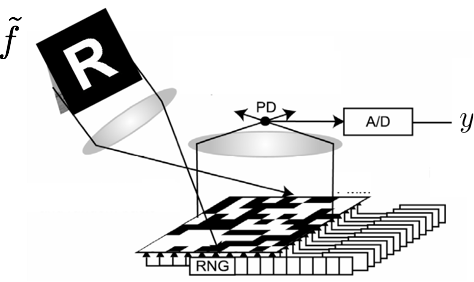
\includegraphics[width=.45\linewidth]{single-pixel/single-pixel-schema}&
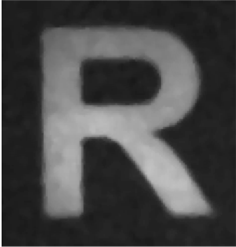
\includegraphics[width=.25\linewidth]{single-pixel/reconstruction-1}&
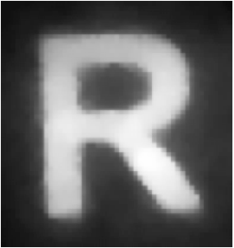
\includegraphics[width=.25\linewidth]{single-pixel/reconstruction-6}\\
Diagram of the device & $f$ & $f^\star$, $P/Q = 6$
\end{tabular}
\caption{Left: diagram of the single-pixel acquisition method.
%
Center: image $f \in \RR^Q$ \guill{ideal} observed in the focal plane of the micro-mirrors.
%
Right: image $f^\star = \Psi x^\star$ reconstructed from observation $y \in \RR^P$ with a compression factor $P / Q = 6$.
\label{fig-single-pixel}}
\end{figure}




%%%%
\subsection{Theoretical Guarantees}

An important feature of this inverse problem is that one can choose, as desired, the configurations of the micro-mirrors, which amounts to saying that one can choose freely the matrix $\Phi \in \{0,1\}^{P \times Q} $. The question is therefore to make the best choice, so that the inverse problem can be solved effectively. If we make the hypothesis that the signal $f$ to be reconstructed is compressible in an orthonormal basis $\Psi$ (that is to say that $f \approx \Psi x_0$ with $M \eqdef \norm{x_0}_0$ small) then several recent works, starting with~\cite{candes2006stable,donoho2006compressed}, showed that method~\eqref{eq-pbm-l1} is effective if $\Phi$ is chosen as a realization of some random matrices. For the single-pixel camera, each $\Phi_{p, n}$ can then be randomly drawn with a probability of $1/2$ for the values $0$ and $1$.
%
In practice, a pseudo-random generator is used, so that both the person who compresses the data and the person who is going to decompress them knows the matrix $\Phi$ perfectly (because they can communicate the seed of the generator).
%
The figure~\ref{fig-single-pixel} (right) shows an example of reconstruction obtained for the case of the single-pixel apparatus with such a random choice of matrix $\Phi$, with $\Psi$ a translation-invariant family of wavelets (see~\cite[Section 5.2]{mallat2009a-wav} for a description of this family).

It has been shown by~\cite{candes2006stable,donoho2006compressed} that there exists a constant $C$ such that if $f = \Psi x_0$ where $x_0$ are the coefficients of the image to be retrieved, where $\Psi$ is an orthogonal basis therefore in particular $Q = N$), and if the number $P$ of measurements satisfies
\eql{\label{eq-cs-contrainte}
\frac{P}{M} \geq C \log\pa{\frac{N}{M}} \qwhereq M \eqdef \norm{x_0}_0
}
then a solution $f^\star = \Psi x^\star$ computed by~\eqref{eq-pbm-l1} tends to $f$ when the $w$ noise tends to $0$ and $\tau$ tends to$ +\infty$. This result is true \guill{with high probability} on the random drawing of the matrix $\Phi$, that is to say a probability tending rapidly towards 1 when $N$ increases. In particular, if there is no noise, $w = 0$, taking $\tau \rightarrow + \infty$, the method makes it possible to find exactly $f$ if $P$ satisfies~\eqref{eq-cs-contrainte}.
%
This theory also allows to take account of \guill{compressible} data, ie if we only assume that $f$ is close to (but not necessarily equal to) $\Psi x_0$ with $M \eqdef \norm{x_0}_0$ small.

Intuitively, this theoretical result means that compressed sampling can do almost \guill{as well} by calculating $\Psi x^\star$ from $y$ (solving~\eqref{eq-pbm-l1}) than a usual compression method (MP3, JPEG , JPEG2000, MPEG, etc.) that would know exactly the $f$ signal and calculate the best approximation $\Psi x_0$ with $M \eqdef \norm{x_0}_0$ coefficients (solving~\eqref{eq-pbm-approx} via the formula~\eqref{eq-expansion-bon}).
%
The precise meaning of the qualifier \guill{equally} corresponds to the $C \log(N/M)$ multiplying factor, which bounds $P/M$. This factor corresponds to the \guill{extra cost} of the compressed sampling method (which calculates $P$ measurements) compared to a usual compression method (which calculates $M$ coefficients).
%
Despite this additional cost, the compressed sampling method has many advantages: saving time and energy (at the same time sampling and compression), \guill{democratic} coding (all $y_n$ coefficients play the same role, and therefore none has a dominant role, unlike the coding of the coefficients of $x_0$ which have an importance proportional to their amplitude), coding automatically encrypted (if $\Phi$ is not known, $f$ can not be found from $y$ ). The value of the $C$ constant depends on the meaning given to \guill{with high probability}. If this probability bears only $\Phi$, but must be true for all $x_0$ (worst case analysis), then it is very large (see~\cite{dossal-laa-09}). If, on the other hand, if the high probability is both on $\Phi$ and $x_0$ (so that the theoretical result is true for almost all the signals) then it can be shown that for example, for $N/P = 4$, we have $C \log (N / M) \sim 4$ (see~\cite{chandrasekaran2012convex}), which remains a significant overhead but is acceptable for some applications.

The \guill{single pixel} camera is a particular application of the compressed sampling technique. Applications to photography are limited because the CCD sensors of cameras are powerful and inexpensive. Compressed sampling is likely to have an impact on applications where measurements are difficult to acquire or costly. Another source of potential applications is medical imaging, for example by magnetic resonance imaging (MRI). In these fields, however, it is impossible to obtain totally random matrices, so that the theory of compressed sampling can not be applied directly. Encouraging results on these applications have however been obtained, see for example~\cite{AdcockBreaking,Chauffert14}.


%%%%%%%%%%%%%%%%%%%%%%%%%%%%%%%%%%%%%%%%%%%%%
\section*{Conclusion}

Recent advances in data analysis have made it possible to extend the scope of compression in order to deal with difficult inverse problems in imaging, but also in other fields (recommendation system, network analysis, etc.). These advances have been made possible by the use of a very broad spectrum of techniques in applied mathematics, covering both harmonic analysis, nonlinear approximation, non-smooth optimization and probability, but also analysis and PDEs (which were not mentioned in this article). Sparse methods associated with $\ell^1$ regularization are only the tip of the iceberg, and more advanced regularizations make it possible to obtain better results by taking into account the complex geometric structures of the data. For more details on these latest advances, we recommend reading the article~\cite{2014-vaiter-ps-review}, as well as visiting the web site \guill{Numerical Tours of Signal Processing}~\cite{2011-peyre-cise}, which features many computer codes to carry out the numerical experiments presented here, as well as many others.

%%%%%%%%%%%%%%%%%%%%%%%%%%%%%%%%%%%%%%%%%%%%%
\section*{Acknowledgments}

I would like to thank Charles Dossal, Jalal Fadili, Samuel Vaiter, St�phane Seuret and the anonymous reviewer for their invaluable help.


